
\newpage
\section{Prototype Design}

\subsection{The Mobile Platform}

`Mobile phone adoption presents us with highly available, contextually aware and interactive platforms'~\cite{article_mhealth}.
Research into designing systems for mobile behaviour change technology, presents us with some implementation design requirements.
Implementing a prototype using these design considerations produces a solid ground for building this system.

\subsection{Design Considerations}

Current mobile systems use apps to interact with users, but a recent study showed apps fall into a low behavioural theory adherence scale~\cite{article_mhealth}.
Research into how to build systems that are theory-based, suggest four main stages for designing mobile health solutions. Conceptualisation, Formative Research and Pretesting,
Pilot trials and Evaluation trials~\cite{article_mhealth}. The first two stages use the Behaviour Change Wheel~\cite{article_behaviour_change_wheel}
(a framework for planning health behaviour interventions), to understand the behaviour, better define the characteristics and form the mobile concept into a prototype.
The pilot trials tests the prototype before it moves to a finalised app with the commitment of a full trial. The final stage tests the finalised app with a wider range of participants.
This project will use these four stages as design steps to build the prototype.

\subsection{Prototype Medium}

This section explores different mediums to develop a prototype, looking into if there is a better method to interact with users than a mobile app. Concludes with developing a Facebook Messenger Chatbot.\newline
\newline
When it comes to mobile phones, users have plenty of options for interaction. A popular choice that has revisited the market are Chatbots, applications that parse questions using Natural Language Processing (NLP) to provide a response, acting as a user interface to expose data. These programs have conversations with users to achieve a goal and are not new inventions. Since 1966~\cite{article_eliza}, Eliza by Joesphs Weizenbaum, used simple expression matching to return a certain response for user trials. In the present day, these applications (commonly referred to as bots, sometimes chatbots), are found integrated into many different apps on the majority of users mobile phones. For example, Facebook Messenger (a popular messaging application) encourages developers to create bots to interact with their users. These bots act as a real person with similar interaction flow, plus a few additional features, such as \textit{Quick Replies} for revealing a list of options to a user. `Quick Replies provide a way to present buttons to the user in response to a message.'~\cite{doc_fb_quick_replies}. However, these bots would not reply like a real person, but rather would only reply if that question was pre-trained using machine learning algorithms. This technology requires the bot to be trained on a large set of data and the majority of use cases would have to be accounted for.\newline
\newline
NLP would enable users to chat to the bot and get a friendly understandable reply. But, would this interaction develop a dependence on the user-chatbot interaction? Would it lead to losing automaticity if the chatbot supported habit formation? NLP will not be used to avoid these potential problems, and instead of natural language processing, the location of the bot (i.e. inside of an existing messaging app), ease of interaction and the additional features (quick replies) will help us easily communicate with a user.\newline
\newline
Another option is a Web App. But a Web App cannot send users reminders, unless it is paired with an app or SMS platform, but this is hard to get a response from a user.\newline
\newline
The below table summarises the available choices for developing a system for our requirements (TODO cite chapter). A mobile app can supply notifications, but for each platform a completely separate app would need to be built and users would need to download the app before it would be available to them.\newline
A single cross-platform app could be constructed to reduce development time and complexity, but still users would need to download the app to start using it.\newline
A web app has the advantage of being available to all users with a web browser (with users being able to save the site to home screen), but without notifications on all platforms (iOS), it won't meet our requirements.\newline
Finally, a chatbot integrated into a popular messaging platform is easily available (if you have the messaging app already installed), simple (the user interface is already supplied), works on any platform the messaging app is available on and has notifications built in.
\renewcommand{\arraystretch}{1.5} % Increase line height of the following tables
\begin{figure}[ht] % ht
\begin{center}
\begin{tabular}{ |p{3.8cm}|p{2.5cm}|p{4cm}|p{2.5cm}|p{2cm}| }
 \hline
 \textbf{} & \textbf{Mobile App} & \textbf{Cross-Platform App} & \textbf{Web App} & \textbf{Chatbot} \\ \hline
 Notifications & \cmark & \cmark & \xmark & \cmark \\ \hline
 Development Time & Long & Medium & Short & Short \\ \hline
 High Availability & \xmark & \xmark & \cmark & \cmark \\ \hline
 Simplicity & \xmark & \xmark & \cmark & \cmark \\
 \hline
\end{tabular}
\end{center}
    \caption{Comparing different prototype mediums.}
    \label{fig:prototype_table}

\end{figure}

From the table above the best method forward is a chatbot. It is already integrated into an existing app users are familer with and (as long as the messaging app is available) works on all platforms.

\subsection{Chatbot Platform}

Discussion about the platform the chatbot should lie onto. Amazon lex \url{https://aws.amazon.com/lex/}. Telegram


Chatbot decided as best method to interact with lots of people easily, after table of pros and cons. Now the real question becomes, would users be able to develop habits with a conversational user interface. Discussion about other types of chatbots, e.g. SMS bot, or Slack bot.

% TODO insert photo of another type of chatbot, e.g. slack bot and SMS bot

Facebook Messenger looks like an attractive option for user interaction:

- Installed on the top 90\% of peoples phones
- Embedded into a service users already use
- Quick replies allows for easy interaction

But, will users differentiate between a bot and a person? Will the text interaction put people off? This thesis aims to answer those questions.

\subsection{Facebook Messenger}

\begin{figure}[ht] % ht
    \centering
    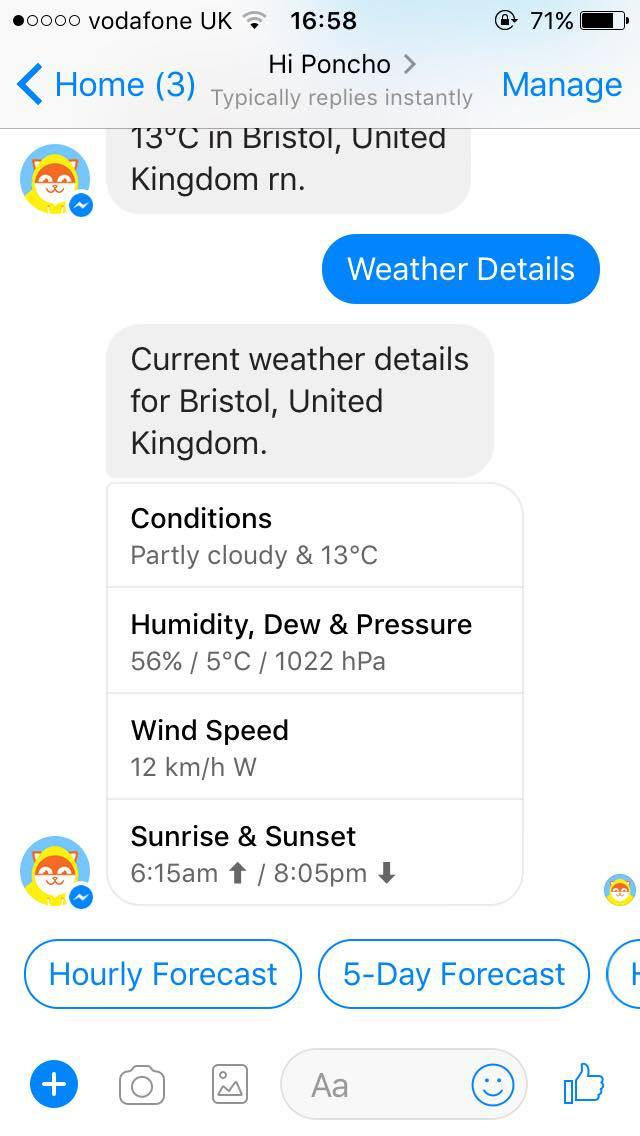
\includegraphics[width=2.5in]{../resources/poncho.jpg}
    \caption{Poncho: An example of Facebook Messenger Weather Chatbot}
    \label{fig:poncho}
\end{figure}

Discussion about the additional features fb messenger has with discussion about previous chatbots.

<photo of UI flow>

<photo of quick replies>

\begin{figure}[ht]
  \centering
  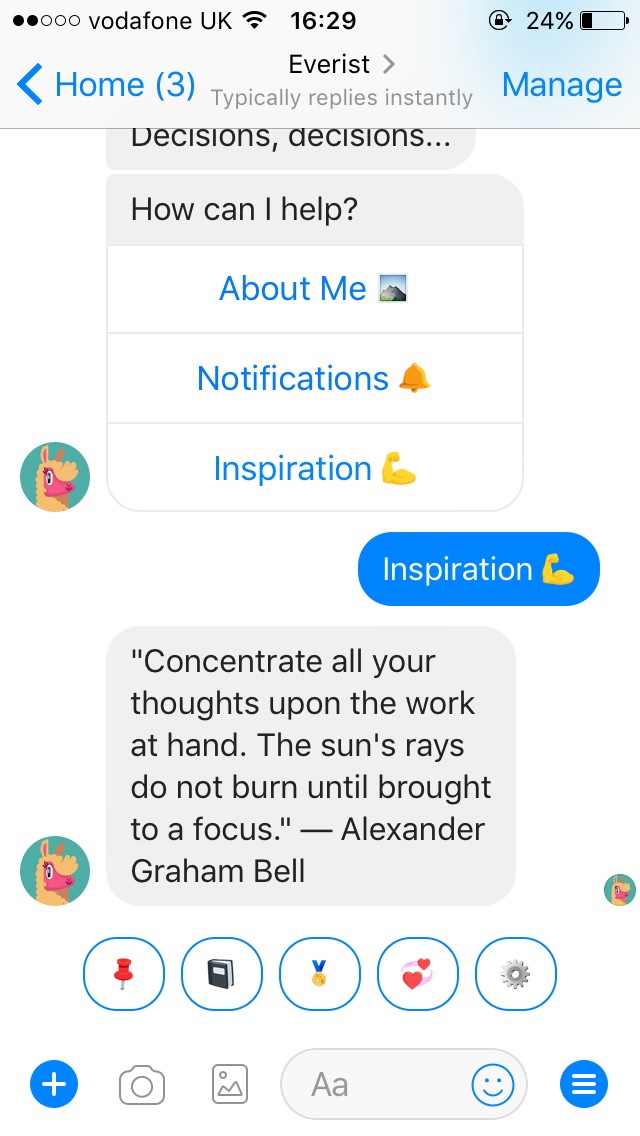
\includegraphics[width=1.9in]{../resources/everist.png}
  \hspace{10px}
  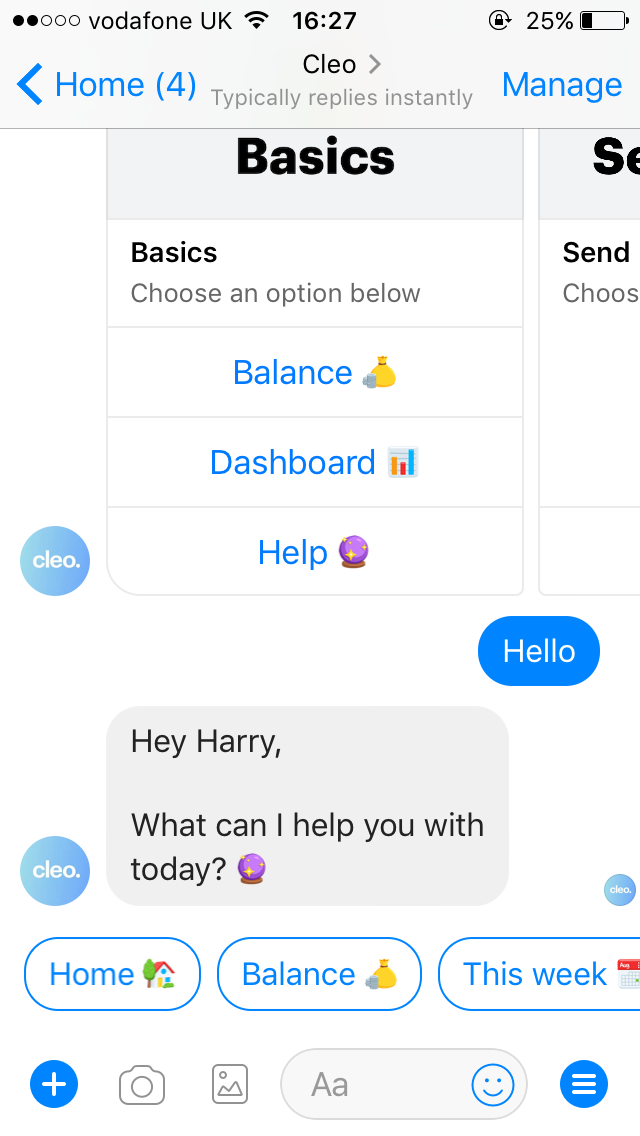
\includegraphics[width=1.9in]{../resources/cleo.png}
  \hspace{10px}
  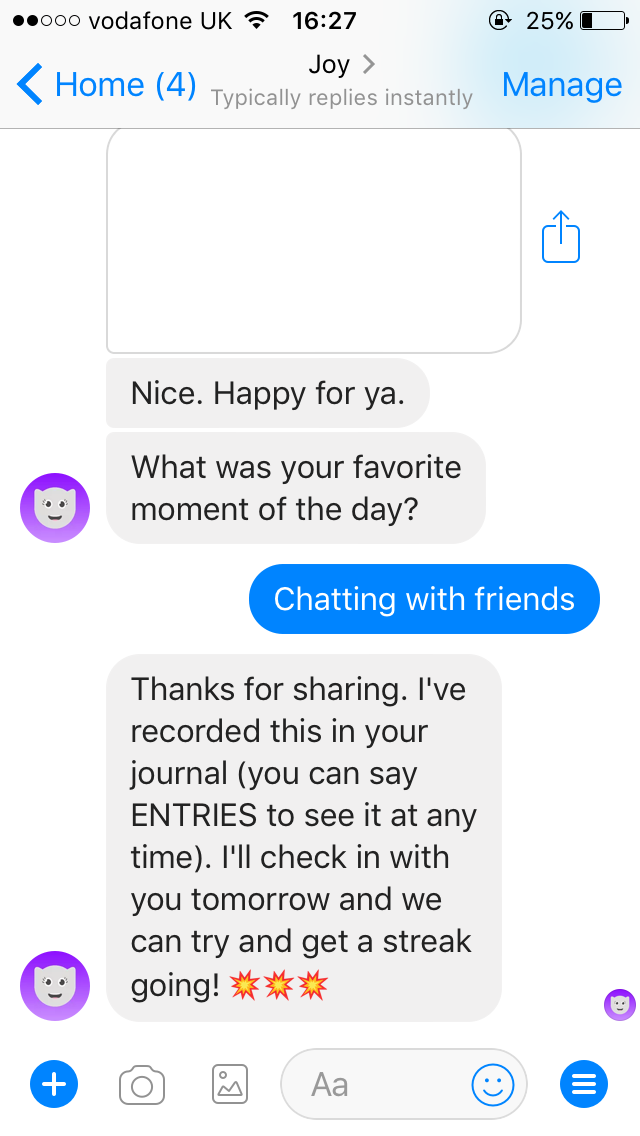
\includegraphics[width=1.9in]{../resources/joy-ai.png}
  \caption{Examples of chatbots performing different actions}
  \label{fig:chatbots_examples}
\end{figure}


\subsection{Supporting Habit Formation}

Discussion about how we can support habit formation using a chatbot in reality.

Paragraph about Gamification elements:
- Gamification elements~\cite{article_free_to_play_making_money_from_games_you_give_away}
- Designing outstanding feedback loops~\cite{website_how_to_design_feedback_loops}


\subsection{Delivering Rewards}

\begin{figure}[ht]
  \centering
  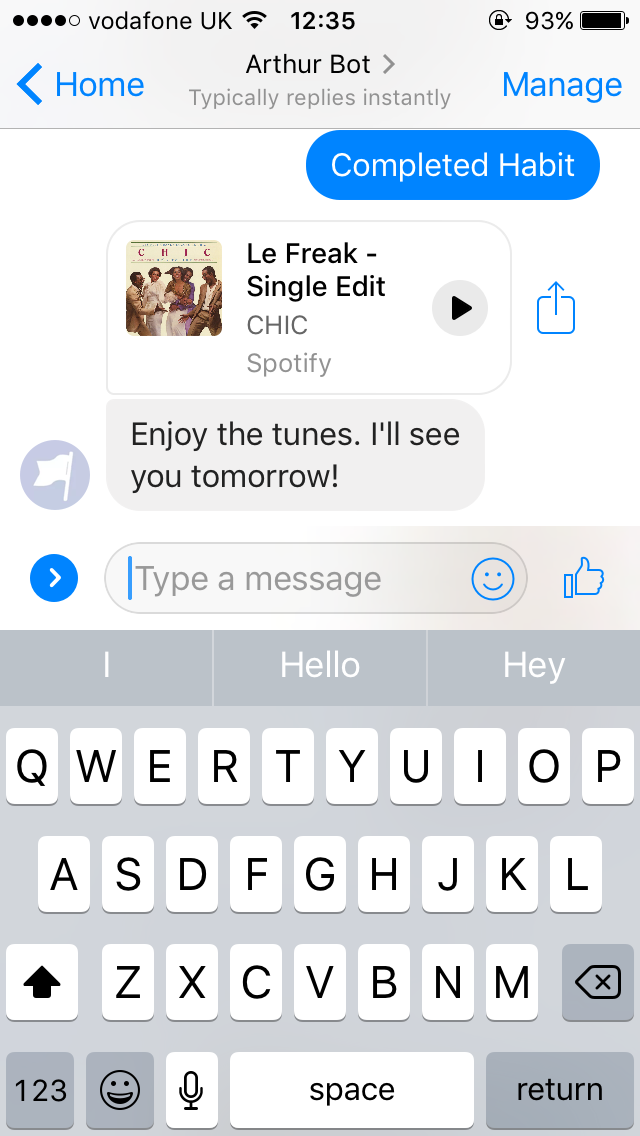
\includegraphics[width=2.1in]{../resources/reward-audio-inline.png}
  \hspace{10px}
  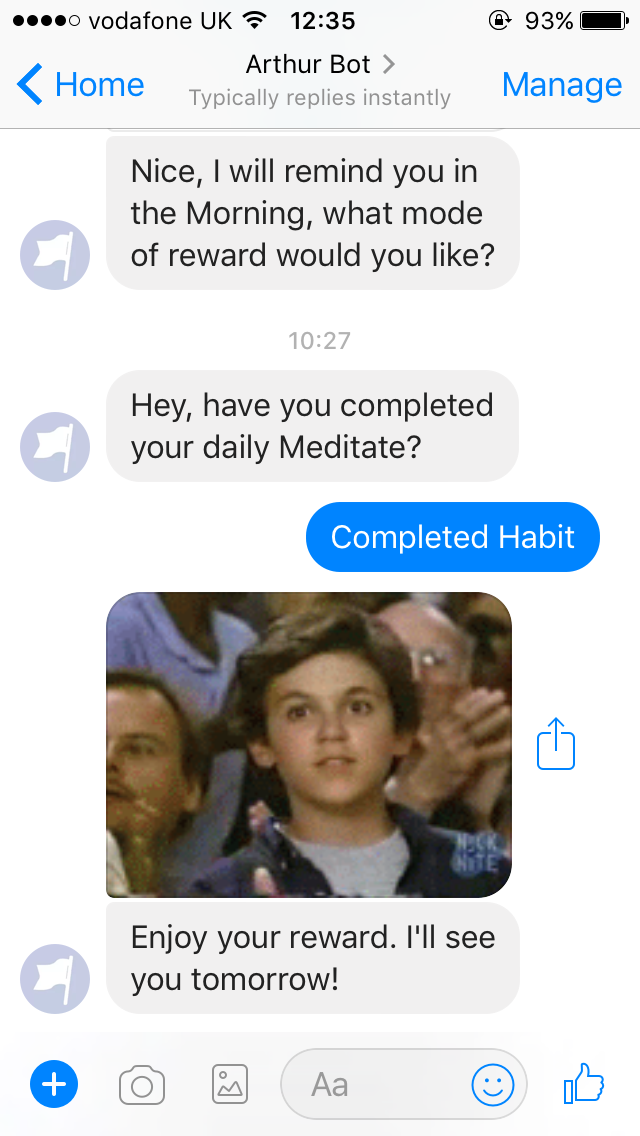
\includegraphics[width=2.1in]{../resources/reward-visual-inline.png}
  \caption{In-line rewards.}
  \label{fig:rewards_inline}
\end{figure}

Discussion about how the rewards will be delivered to the users. In-line verses same screen. How interaction is handled. Concludes with exactly how rewards will be handled in design way, brief discussion about vibration and how it would not work.

\begin{figure}[ht]
  \centering
  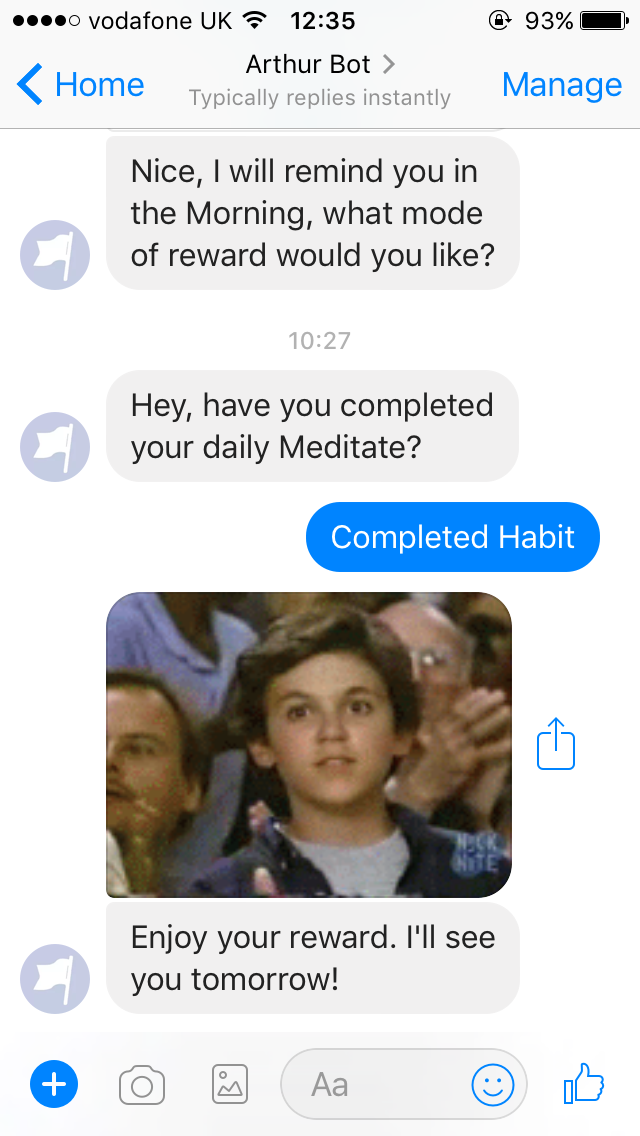
\includegraphics[width=2.1in]{../resources/reward-visual-inline.png}
  \hspace{10px}
  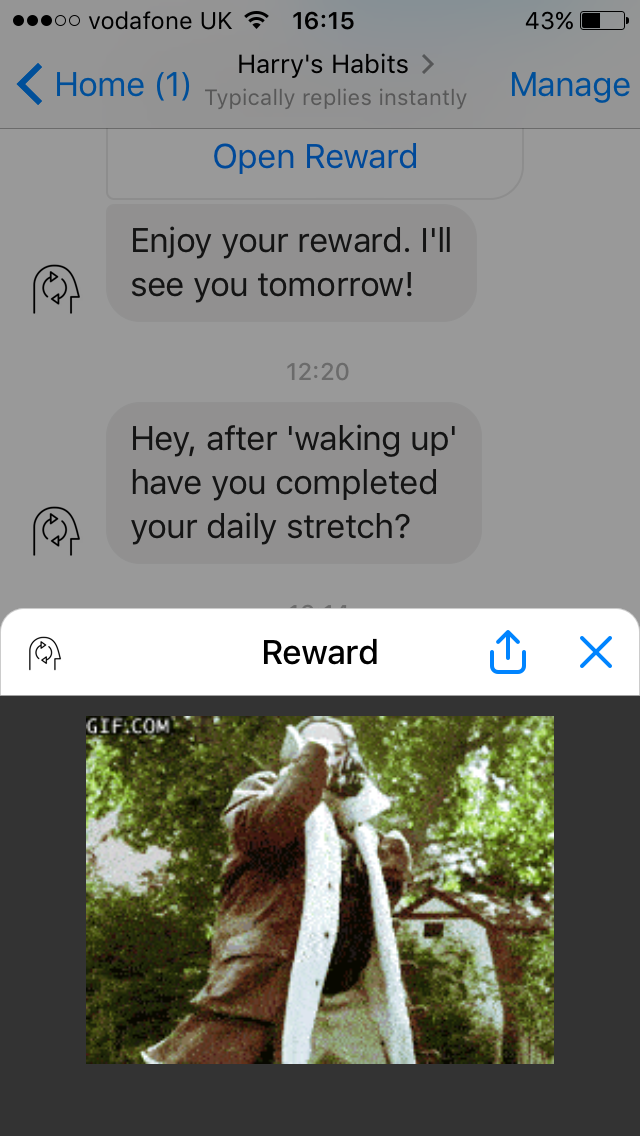
\includegraphics[width=2.1in]{../resources/reward-visual-2.png}
  \caption{In-line visual rewards verses separate.}
  \label{fig:rewards_inline_v_website}
\end{figure}

The types of rewards are separated into three categories, visual, auditory and combined visual-auditory. Different types of these rewards will be experimented with,
and test if they provide user satisfaction. These rewards will be displayed to the user within the chatbot after they complete their habit.
For a playful prototype, visual rewards will be light-hearted gifs and auditory rewards will be selected to match the gifs.

\begin{figure}[ht]
  \centering
  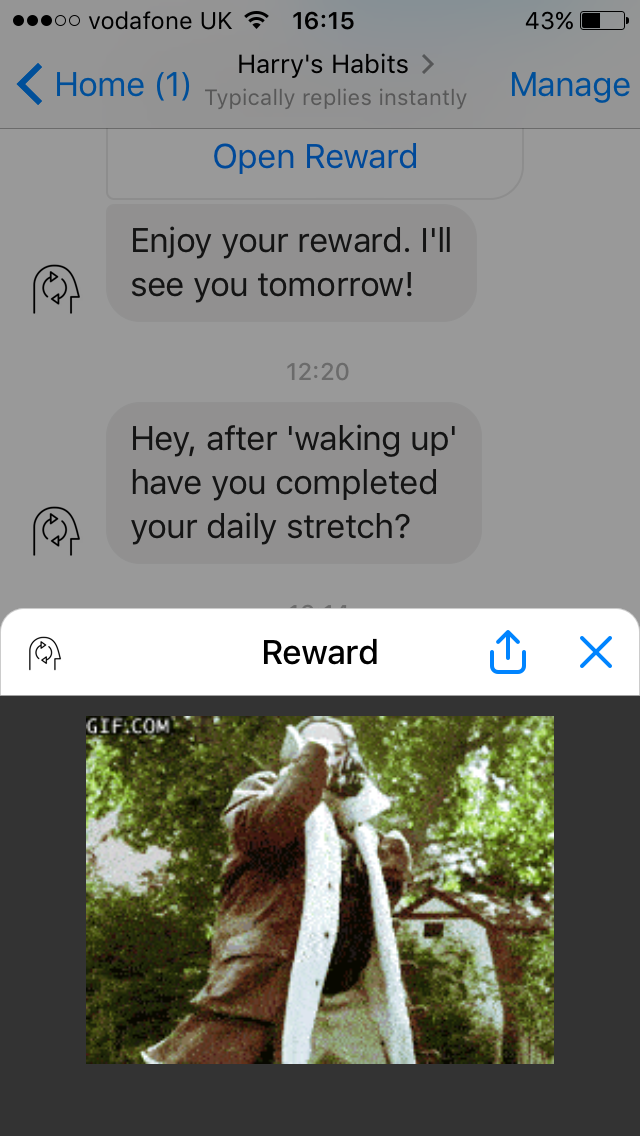
\includegraphics[width=2.1in]{../resources/reward-visual-2.png}
  \hspace{10px}
  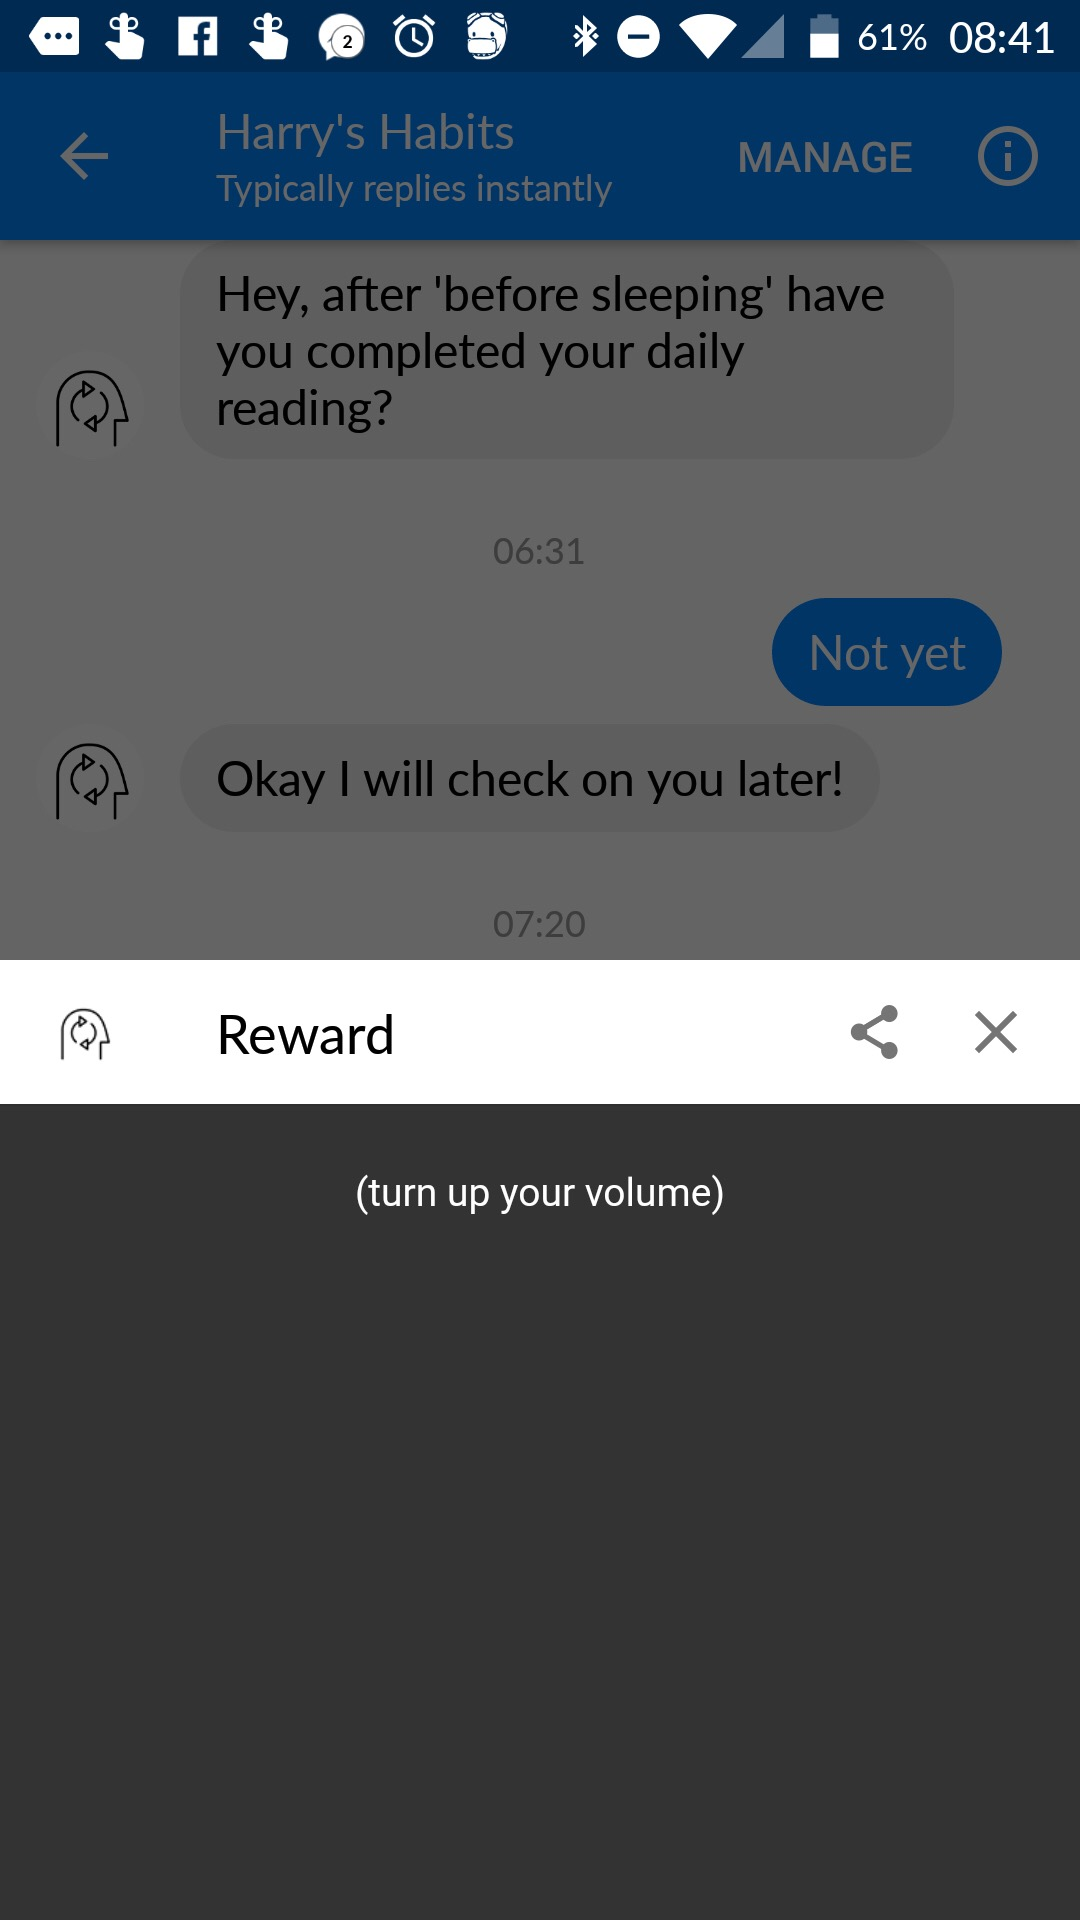
\includegraphics[width=2.1in]{../resources/reward-audio.png}
  \caption{Consistency between every reward, even across devices.}
  \label{fig:rewards_consistency}
\end{figure}

\subsection{Technical Limitations}
Vibration discussion: - A.P.I. sets wearable alarm - Wearable (fitbit) issues and tracks alarm times
Audio autoplay limitations:

\subsection{User Flow}

Full user interaction from setup to completing a reward.

\begin{itemize}
  \item \textbf{Setup}
  \begin{itemize}
    \item Setup the bot via a messaging platform, such as Facebook messenger.
    \item User chooses an existing habit they would like to develop.
    \item User supplies an existing context to integrate their new habit into.
    \item User supplies a time the existing context occurs.
  \end{itemize}
  \item \textbf{Trigger}
  \begin{itemize}
    \item At the time of the existing context, the user should perform their chosen habit.
    \item The user receives a notification after the chosen time, that asks if they managed to complete their habit, or if they need more time.
    \item If they need more time, the notification will \textit{snooze} for about an hour and be sent again.
    \item If users regularly snooze they will be asked if their existing context time would like to change.
    \item If users say they have completed their habit, they will receive a reward.
  \end{itemize}
  \item \textbf{Reward}
  \begin{itemize}
    \item Users will press a button that will take them to a website so for each modality they can consistently experience their reward.
    \item User will receive a reward (which represents success) from one of the following modalities:
    \item Visual: A video with no sound
    \item Audio: A soundtrack
    \item Visual and Audio: A video with sound
  \end{itemize}
\end{itemize}

\section{Prototype Implementation}

Abstract implementation overview of user and chatbot discussion.

<photo sketched>
  % [app] -------> (Database) -----> at certain time ---> Send notification to trigger type of reward
  % [ big button that says track]
  % taskname textbox

% Flow diagram style
\tikzstyle{startstop} = [rectangle, rounded corners, minimum width=3cm, minimum height=1cm,text centered, draw=black, fill=red!30]
\tikzstyle{io} = [trapezium, trapezium left angle=70, trapezium right angle=110, minimum width=3cm, minimum height=1cm, text centered, draw=black, fill=blue!30]
\tikzstyle{process} = [rectangle, minimum width=3cm, minimum height=1cm, text centered, draw=black, fill=orange!30]
\tikzstyle{decision} = [diamond, minimum width=3cm, minimum height=1cm, text centered, draw=black, fill=green!30]
\tikzstyle{arrow} = [thick,->,>=stealth]

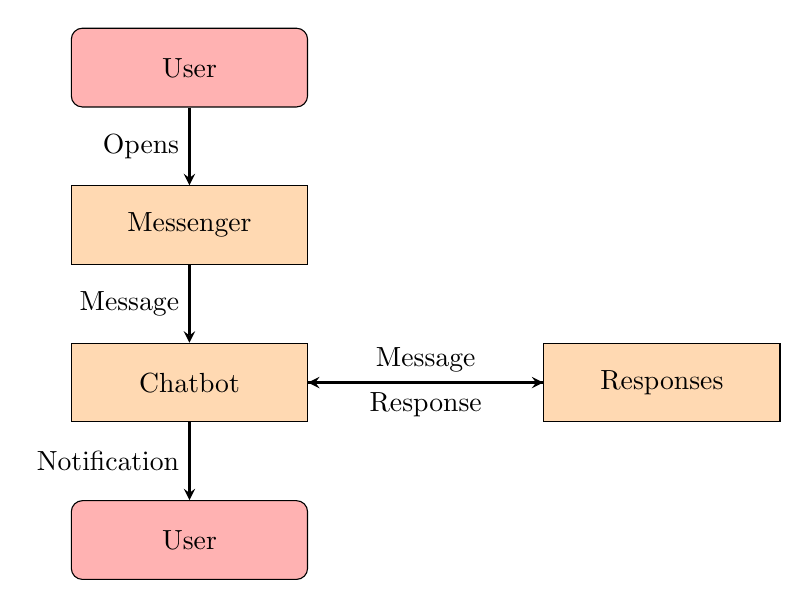
\begin{tikzpicture}[node distance=2cm]
  \node (user) [startstop] {User};
  \node (fbmsgr) [process, below of=user] {Messenger};
  \node (chatbot) [process, below of=fbmsgr] {Chatbot};
  \node (responses) [process, right of=chatbot, xshift=4cm] {Responses};
  \node (userend) [startstop, below of=chatbot] {User};

  \draw [arrow] (user) -- node[anchor=east] {Opens} (fbmsgr);
  \draw [arrow] (fbmsgr) -- node[anchor=east] {Message} (chatbot);
  \draw [arrow] (chatbot) -- node[anchor=south] {Message} (responses);
  \draw [arrow] (responses) -- node[anchor=north] {Response} (chatbot);
  \draw [arrow] (chatbot) -- node[anchor=east] {Notification} (userend);
\end{tikzpicture}

\subsection{Platform}

Language consideration, nodejs, java, other types, talk about heroku, hosting provider. Hosting provider.
Database provider discussion, integration, airtable,

\subsection{Detailed Overview}

Architecture Component overview w diagram\newline
Chatbot function overview w diagram\newline
Implementation limitations\newline
Scheduler\newline
Free text input\newline

\subsection{Implementation Issues}

Go through all meetings and list issues here


\newpage
